
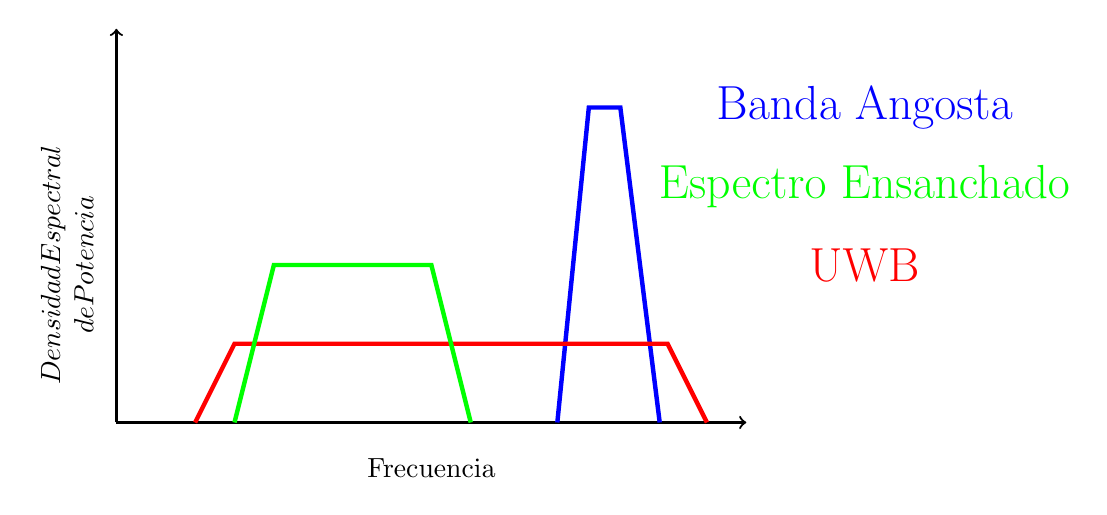
\begin{tikzpicture}

	\coordinate (O) at (0,0);
	
	\draw[thick, ->] (O) -- (8.0,0);
	\node[anchor = base] at (4, -0.7){Frecuencia};
	
	\draw[thick, ->] (O) -- (0,5.0);
	\node[anchor = base, rotate = 90] at (-0.5,2) {{$\begin{array}{cc} \text{Densidad Espectral} \\ \text{de Potencia}\end{array}$}};
	
	\draw[blue, ultra thick] plot coordinates {(5.6, 0) (6.0, 4) (6.4, 4) (6.9,0)};
	
	\draw[red, ultra thick] plot coordinates {(1,0) (1.5,1) (7,1) (7.5,0)};
	
	\draw[green, ultra thick] plot coordinates {(1.5, 0) (2,2) (4,2) (4.5,0)};
	
	\node[blue] at (9.5, 4) {\LARGE Banda Angosta};
	\node[green] at (9.5,3) {\LARGE Espectro Ensanchado};
	\node[red] at (9.5, 2) {\LARGE UWB};

\end{tikzpicture}